%%class
\documentclass{iaesarticle3}

%%required package. add for your convenient, but do not remove the initial
\usepackage{amsmath, amsfonts, amssymb, float, fancyhdr}
\usepackage[scaled]{uarial}
\usepackage[figuresright]{rotating}
\usepackage{authblk, graphicx, indentfirst, lastpage, lipsum}
\setlength{\affilsep}{0cm}
\renewcommand\Authfont{\normalsize}
\renewcommand\Affilfont{\normalfont\small}
\usepackage{subfig, caption, epstopdf}
\usepackage[left=3cm, right=3cm, top=3cm, bottom=3cm, includefoot]{geometry}
\usepackage{caption}
\captionsetup{labelsep=period}
\usepackage{titlesec}
\titleformat{\section}
  {\normalfont\normalsize\bfseries}{\thesection}{1em}{}
\titlespacing*{\section}{0cm}{0.7cm}{0cm}
\titlespacing*{\subsection}{0cm}{0.5cm}{0cm}

%%Additional package
\usepackage{booktabs, array, multirow, multicol}

%%leave copyright info to the editor
\CopyrightLine[Copyright]{2018}{Universitas Ahmad Dahlan. All rights reserved.}

%%author
\author[1]{\bfseries Yudy Purnama*}
\author[2]{\bfseries Fergyanto E. Gunawan}

%%author's affiliation
\affil[1]{Computer Science Department, School of Computer Science}
\affil[2]{Industrial Engineering Department}
\affil[2]{BINUS Graduate Program - Master of Industrial Engineering}
\affil[ ]{Bina Nusantara University, Jakarta, Indonesia 11480}
\affil[ ]{*Corresponding Author, email: \textsuperscript{1}ypurnama@binus.edu, \textsuperscript{2}fgunawan@binus.edu}

%%title and shortitle (for footer)
\title{Vibration-Based Damaged Road Classification Using Artificial Neural Network}
\shorttitle{Vibration-Based Damaged Road Classification Using Artificial ... (Yudy Purnama)}

%%starting
\begin{document}
\setcounter{page}{2179}

%%indentation. do not change
\setlength{\parindent}{1.27cm}

%%header and footer setting. do not change
\pagestyle{fancy}
\fancyhfoffset{0cm}


%%journal info
\journalname{TELKOMNIKA}
\journalshortname{TELKOMNIKA}
\revhistory{Received October 14, 2017; Revised May 20, 2018; Accepted June 13, 2018}
\vol{16}
\no{5}
\months{October}
\years{2018}
%\issn{2302-4046}
\issn{1693-6930}

%%build title
\maketitle

\begin{abstract}
\textit{\indent
%% Text of abstract
It is necessary to develop an automated method to detect damaged road because
manually monitoring the road condition is not practical. Many previous studies
had demonstrated that the vibration-based technique has potential to detect
damages on roads. This research explores the potential use of Artificial Neural
Network (ANN) for detecting road anomalies based on vehicle accelerometer data.
The vehicle is equipped with a smart-phone that has a 3D accelerometer and
geo-location sensors. Then, the vehicle is used to scan road network having
several road anomalies, such as, potholes, speedbump, and expansion joints. An
ANN model consisting of three layers is developed to classify the road
anomalies. The first layer is the input layer containing six neurons. The
numbers of neurons in the hidden layer is varied between one and ten neurons,
and its optimal number is sought numerically. The prediction accuracy of 84.9\%
is obtained by using three neurons in conjunction with the maximum acceleration
data in $x$, $y$, and $z$-axis. The accuracy increases slightly to 86.5\%, 85.2\%, and
85.9\% when the dominant frequencies in $x$, $y$, and $z$-axis, respectively, are taken
into account beside the previous data.
%%
}
\end{abstract}

\begin{keyword}
\textit{
%%write keyword here. separate by comma (,)
Damaged Road, Vibration-based, Accelerometer, Smart-phone, Artificial Neural Network
%%
}
\end{keyword}


%% main text

%%SECTION I
%%=============================================================================================
\section{Introduction}
\label{}
According to Law of the Republic of Indonesia, No. 22, Year 2009 about Road Traffic and Transportation (\textit{Undang-undang Republik Indonesia Nomor 22 Tahun 2009 Tentang Lalu Lintas dan Angkutan Jalan}) Article 24 Section (1), road
administrator or government shall immediately and should repair any damaged road
that could lead to traffic accidents \cite{uu22}. Furthermore, Section 2 of the
law states that in the case that the damaged road cannot be repaired, the road
administrator is obliged to put sign(s) on the damaged roads to prevent traffic
accidents. In the case that traffic accidents occurred because the road
administrator does not immediately repair the damaged road, they can be
imprisoned or fined. The duration of imprisonment varies between six months up
to five years. The amount of fine varies between 12 millions up to 120 millions
rupiah, depending on the victim condition.
\par Road administrator needs a method to detect damaged road. It is necessary
to develop an automated method to detect damaged road manually because
monitoring the road condition is not practical. Several research efforts towards
automating damaged road detection have been undertaken. There were 3D pavement
reconstruction methods \cite{jiaqiu2009research, jog2012pothole}  and laser
imaging method \cite{yu2011pavement}. Those methods required special devices,
making them less economical and difficult to implement in real situation. There
were also vibration-based approach using acceleration sensor available on
smart-phones \cite{eriksson2008pothole, vittorio2014automated}.
\par The previous studies had demonstrated that vibration technique has
potential to detect damaged road \cite{de2007public, gunawan2015vibratory}.
However, those studies were only able to differentiate damaged roads from
un-damaged one, without ability to distinguish the types of the road anomaly. In
this research, we intend to develop a road anomaly classification. Data are
collected by using a 3D accelerometer in Android smart-phone. The accelerometer
records the vehicle vibration. Our system can detect few types of  road anomaly.
If one is found, then our artificial neural network system will classify its
type whether pothole or speed-bump.
%%=============================================================================================

%%SECTION 2
%%=============================================================================================
\section{Research Method}
\label{}
\subsection{Relevant Works}
The size of road network that increases massively demands an automatic road
monitoring system. However, the system is hard to develop considering the
complexity of the road conditions. Fortunately, the roadways and mobile phone
networks have grown simultaneously in emerging economies. Mukherjee and Majhi
\cite{mukherjee2016characterisation} demonstrated the capability of using
smart-phone that has accelerometers and position sensors. This capability can be
useful for autonomous monitoring roads.
The ability of the smart-phone in recording accelerations reliably is
demonstrated.
\par Gunawan et al. \cite{gunawan2015vibratory} performed similar experiment
that utilized a smart-phone which was enriched with a 3D accelerometer sensor
and geo-location sensor. The smart-phone installed in a vehicle. Their study
found that whenever a vehicle crosses a pothole, it will vibrate significantly
in $z$ and $x$ directions. Data collected from the pothole case were statistically
deviated from the normal road and the bump road cases which showing potential
for classification purpose.

\subsection{Motion Sensors on Android Phone}
Motion sensors on Android Phone return a multi-dimensional array of data
measured by each sensor at an instance of time \cite{website:android-motion}.
The accelerometer sensor measure accelerations in three directions, namely, $x$,
$y$, and $z$-axis. The orientations of those axis on a smart-phone is depicted
in Figure \ref{fig:Accelerometer}.
The results of the orientations on the accelerometer responses are the
following. If the device is pushed on the left side (device moves to the right),
the $x$ acceleration value will be positive.
\par If the device is pushed on the bottom side (device moves away from user),
the y acceleration value will be positive.
If the device is pushed toward the sky with an acceleration of
$A\,\text{m/s}^2$, then the $z$ acceleration value equal to
$A+9.81\,\text{m/s}^2$, which corresponds to the acceleration of the device
($A\,\text{m/s}^2$) minus the acceleration of gravity ($-9.81\,\text{m/s}^2$).
\par The device on stationary condition will have an acceleration value of
$+9.81\,\text{m/s}^2$, which corresponds to the acceleration of the device
($0\,\text{m/s}^2$) minus the acceleration of gravity ($-9.81\,\text{m/s}^2$).

\begin{figure}[b]
	\centering
	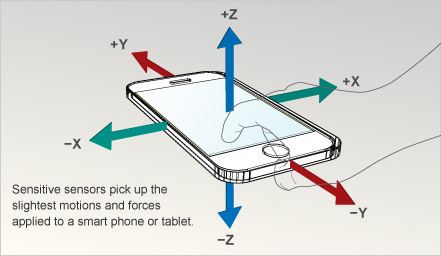
\includegraphics[scale=0.5]{figures/Accelerometer.png}
	\caption{The orientation of the three axes on Android smart-phone \protect\cite{website:android-motion}.}
	\label{fig:Accelerometer}
\end{figure}

\subsection{Vibration-based Method}
Most road anomalies can be characterized as high-energy events in the
acceleration data, yet not all events are road anomalies. Another thing such as
road fixtures (railroad crossings and expansion joint) can generate significant
acceleration impulse. Passengers slamming the door or driver braking suddenly
can also produce high energy events.
\par Eriksson et al. \cite{eriksson2008pothole} and Gunawan et al.
\cite{gunawan2015vibratory} used vehicle acceleration data as the main source.
Smart-phone which is enriched with a 3D accelerometer sensor and geo-location
sensor is installed into the vehicle.
\par Figure \ref{fig:PotholeDetectionFlowchart} shows the pothole detection
flowchart used. The detection method would be as follow:

\begin{enumerate}
  	\itemsep 0em
	\item Vehicle velocity will be evaluated. If it is too low, this stream of data will be ignored, and next new stream of data will be evaluated. This process will be repeat until the stream data satisfied the requirement
	\item Apply high-pass filter to remove acceleration, braking, or turn events
	\item $z$ direction acceleration ($a_z$) will be evaluated against a threshold ($t_z$). This stream data would be further processed if maximum of $a_z$ ($a_z^{\text{max}}$) exceeds ($t_z$); Otherwise new data stream will be evaluated (back to step 1).
	\item Calculate the largest value of x direction acceleration data ($a_x$) within the time interval centered at the time of $a_x^{\text{max}}$ occurring. The time interval may vary (32, 64, or 128). This extreme value will be checked against a threshold ($t_x$). Similar to previous step, if $a_x^{\text{max}} < t_x$, this stream data will be ignored and new one will be tested (back to step 1).
	\item Last step is to reject any data if $t_z^{\text{max}} < t_s . v$, where $t_s$ is threshold and $v$ is the vehicle traveling velocity.
\end{enumerate}

\begin{figure}[b]
	\centering
	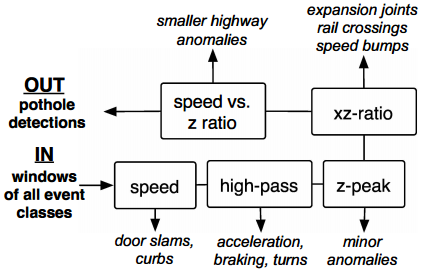
\includegraphics[scale=0.75]{figures/PotholeDetectionFlowchart.png}
	\caption{Pothole Detection Flowchart \protect\cite{eriksson2008pothole}.}
	\label{fig:PotholeDetectionFlowchart}
\end{figure}


\subsection{Data Collection}
Road anomaly can be defined as abnormality of the road condition from what it
supposed. There are several kinds of road anomaly such as damaged road (pot hole
existence), speed bump, railroad crossing, or expansion joint. This research
will focus on providing a method to detect road anomaly in real time and further
classify the types of the road anomaly. There are several things to be prepared
before data collection can be performed: smart-phone, vehicle, accelerometer
data and the road anomaly it selves.
\par
Smart-phone and vehicle: In this research, two smart-phone devices will be used:
Device A and B. Device A will be placed on the card dashboard, while the device
B will be placed in the middle of the car floor close to the back passenger
Accelerometer data: Third party software that will be used to record the vehicle
acceleration data. This application will record the acceleration data and save
it in a .csv file.
\par
Road anomaly: There are four kinds of road condition that will be recorded:
normal, road with pothole, road with speed bump, and road with expansion joint.


\subsection{Feature Extraction}
Raw accelerometer data may not be directly used. These anomalies data are mixed
with �noise� data, such as passengers slamming the door or driver braking
suddenly that can also produce high energy events. There are several steps
before features can be extracted from the raw data, they are:

\begin{enumerate}
	\itemsep 0em
	\item Zero Shift: The purpose of this process to shift each acceleration data ($x$, $y$, and $z$) values in data to zero. All acceleration data are subtracted by theirs median.
	\item Savitzky-Golay Filter: The purpose of this step is to remove �noise� from this acceleration data. The polynomial order used in this filter is one with frame size of 41.
	\item Determine $z$ acceleration peak point: The moment vehicle wheel hit the damaged road, the $z$ acceleration will reach its peak. This point will becomes the median value of cutting window of data. Number 32 chosen as the size of the window to cover more point in time span, because there is a possibility that the peak window can be missed. Therefore data used are 65 points span between ($z_\text{max}-32$) and ($z_\text{max}+32$).
	\item Hamming Window and Fast Fourier Transform: Fourier Transform is implicitly applied to an infinitely repeating signal. Sometimes the start and end of the finite sample signal do not match, hence make it looks like a discontinuity in the signal. Applying Hamming Window makes sure that the ends match up while keeping everything reasonably smooth. Sixty-five points that has been acquired before will be applied with Hamming Window.
\end{enumerate}

\subsection{ANN Model for Classification}
ANN is used as classification method because its
capability to learn from examples and capture the functional relationships among
the hard description of data. The network will be a Multilayer back-propagation
network. This network will use Sigmoid as its activation function.Network
parameter such as percentage of training data and number of hidden layers will
be changed and tested several times to achieve the optimal result.
\par
Figure \ref{fig:ANNModel} shows the ANN model used in this study. After pre-processing, there are
five input nodes: maximum $x$ acceleration data ($a^{\text{max}}_{x}$), maximum $z$ acceleration data ($a^{\text{max}}_{z}$),
dominant frequency of $x$ acceleration ($f^{\text{dom}}_{x}$), dominant frequency of y acceleration ($f^{\text{dom}}_{y}$), and
dominant frequency of $z$ acceleration ($f^{\text{dom}}_{z}$). The output node would be chosen from four
available classes of the road condition: normal, speed-bump, pothole, and
expansion joint.

\begin{figure}[b]
	\centering
	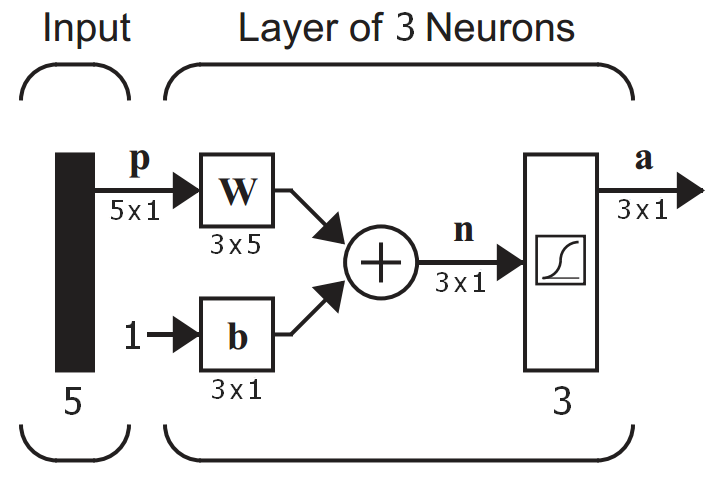
\includegraphics[scale=0.4]{figures/ANNModel.png}
	\caption{A neural network model with five neurons in the input layer and three neurons in the hidden layer}
	\label{fig:ANNModel}
\end{figure}

Table \ref{tab:ANNParameter} shows the parameter of neural network used in this study. If there are
500 data, and ANN set to 10\% training set size and 50\% validation set size, data
composition will be: 50 testing data (randomly chosen), 225 testing data, and
225 validation data.
\par
There are two separated experiments. First experiment is to determine the
reliable sample size: This process determines minimum portion of training data
needed to achieve desired result. Training data portion will be increased
gradually with increment of 10\% until 90\% portion of training data. Every
multiple of 10\%, the data set will be classified a hundred times. The optimal
training data portion will be used in the second process.
\par
The second process is determining the optimum number of Neurons: Using
previously obtained optimal parameter, number of neurons in the hidden layer
will be changed from 2 up to 9. Each variation will be run for 100 times
classification process.

\begin{table}[t]
	\centering
	\caption{Neural Network Parameters Used in This Study.}
	\begin{tabular}[c]{|c|c|}
		\hline
		\textbf{Parameter} & \textbf{Value}
		\\
		\hline
		Activation function & Sigmoid		
		\\
		\hline
		Learning rate & 0.3
		\\
		\hline
		Momentum & 0.2
		\\
		\hline
		Training time & 10000
		\\
		\hline
		Number of neuron in the hidden layers & 2--9
		\\
		\hline
		Training set size & 10--90\%
		\\
		\hline
		Validatian set size & 50\%
		\\
		\hline		
	\end{tabular}
	\label{tab:ANNParameter}
\end{table}

%%=============================================================================================


%%SECTION 3
%%=============================================================================================
\section{Result and Analysis}

\subsection{Typical Acceleration Data}
This section shows how each road anomaly affects the accelerometer data. Figure
\ref{fig:TypicalNormal} shows acceleration data when a vehicle crosses a normal
road. The best indicator is that $z$ acceleration tends to stay at gravity
acceleration which is $+9.81\,\text{m/s}^2$. Using this information can be
concluded that vehicle crosses normal road will have its $z$ acceleration
relatively stays at $+9.81\,\text{m/s}^2$. Any rise or fall from this value is
the indicator of road anomaly.

\begin{figure}[!hb]
	\centering
	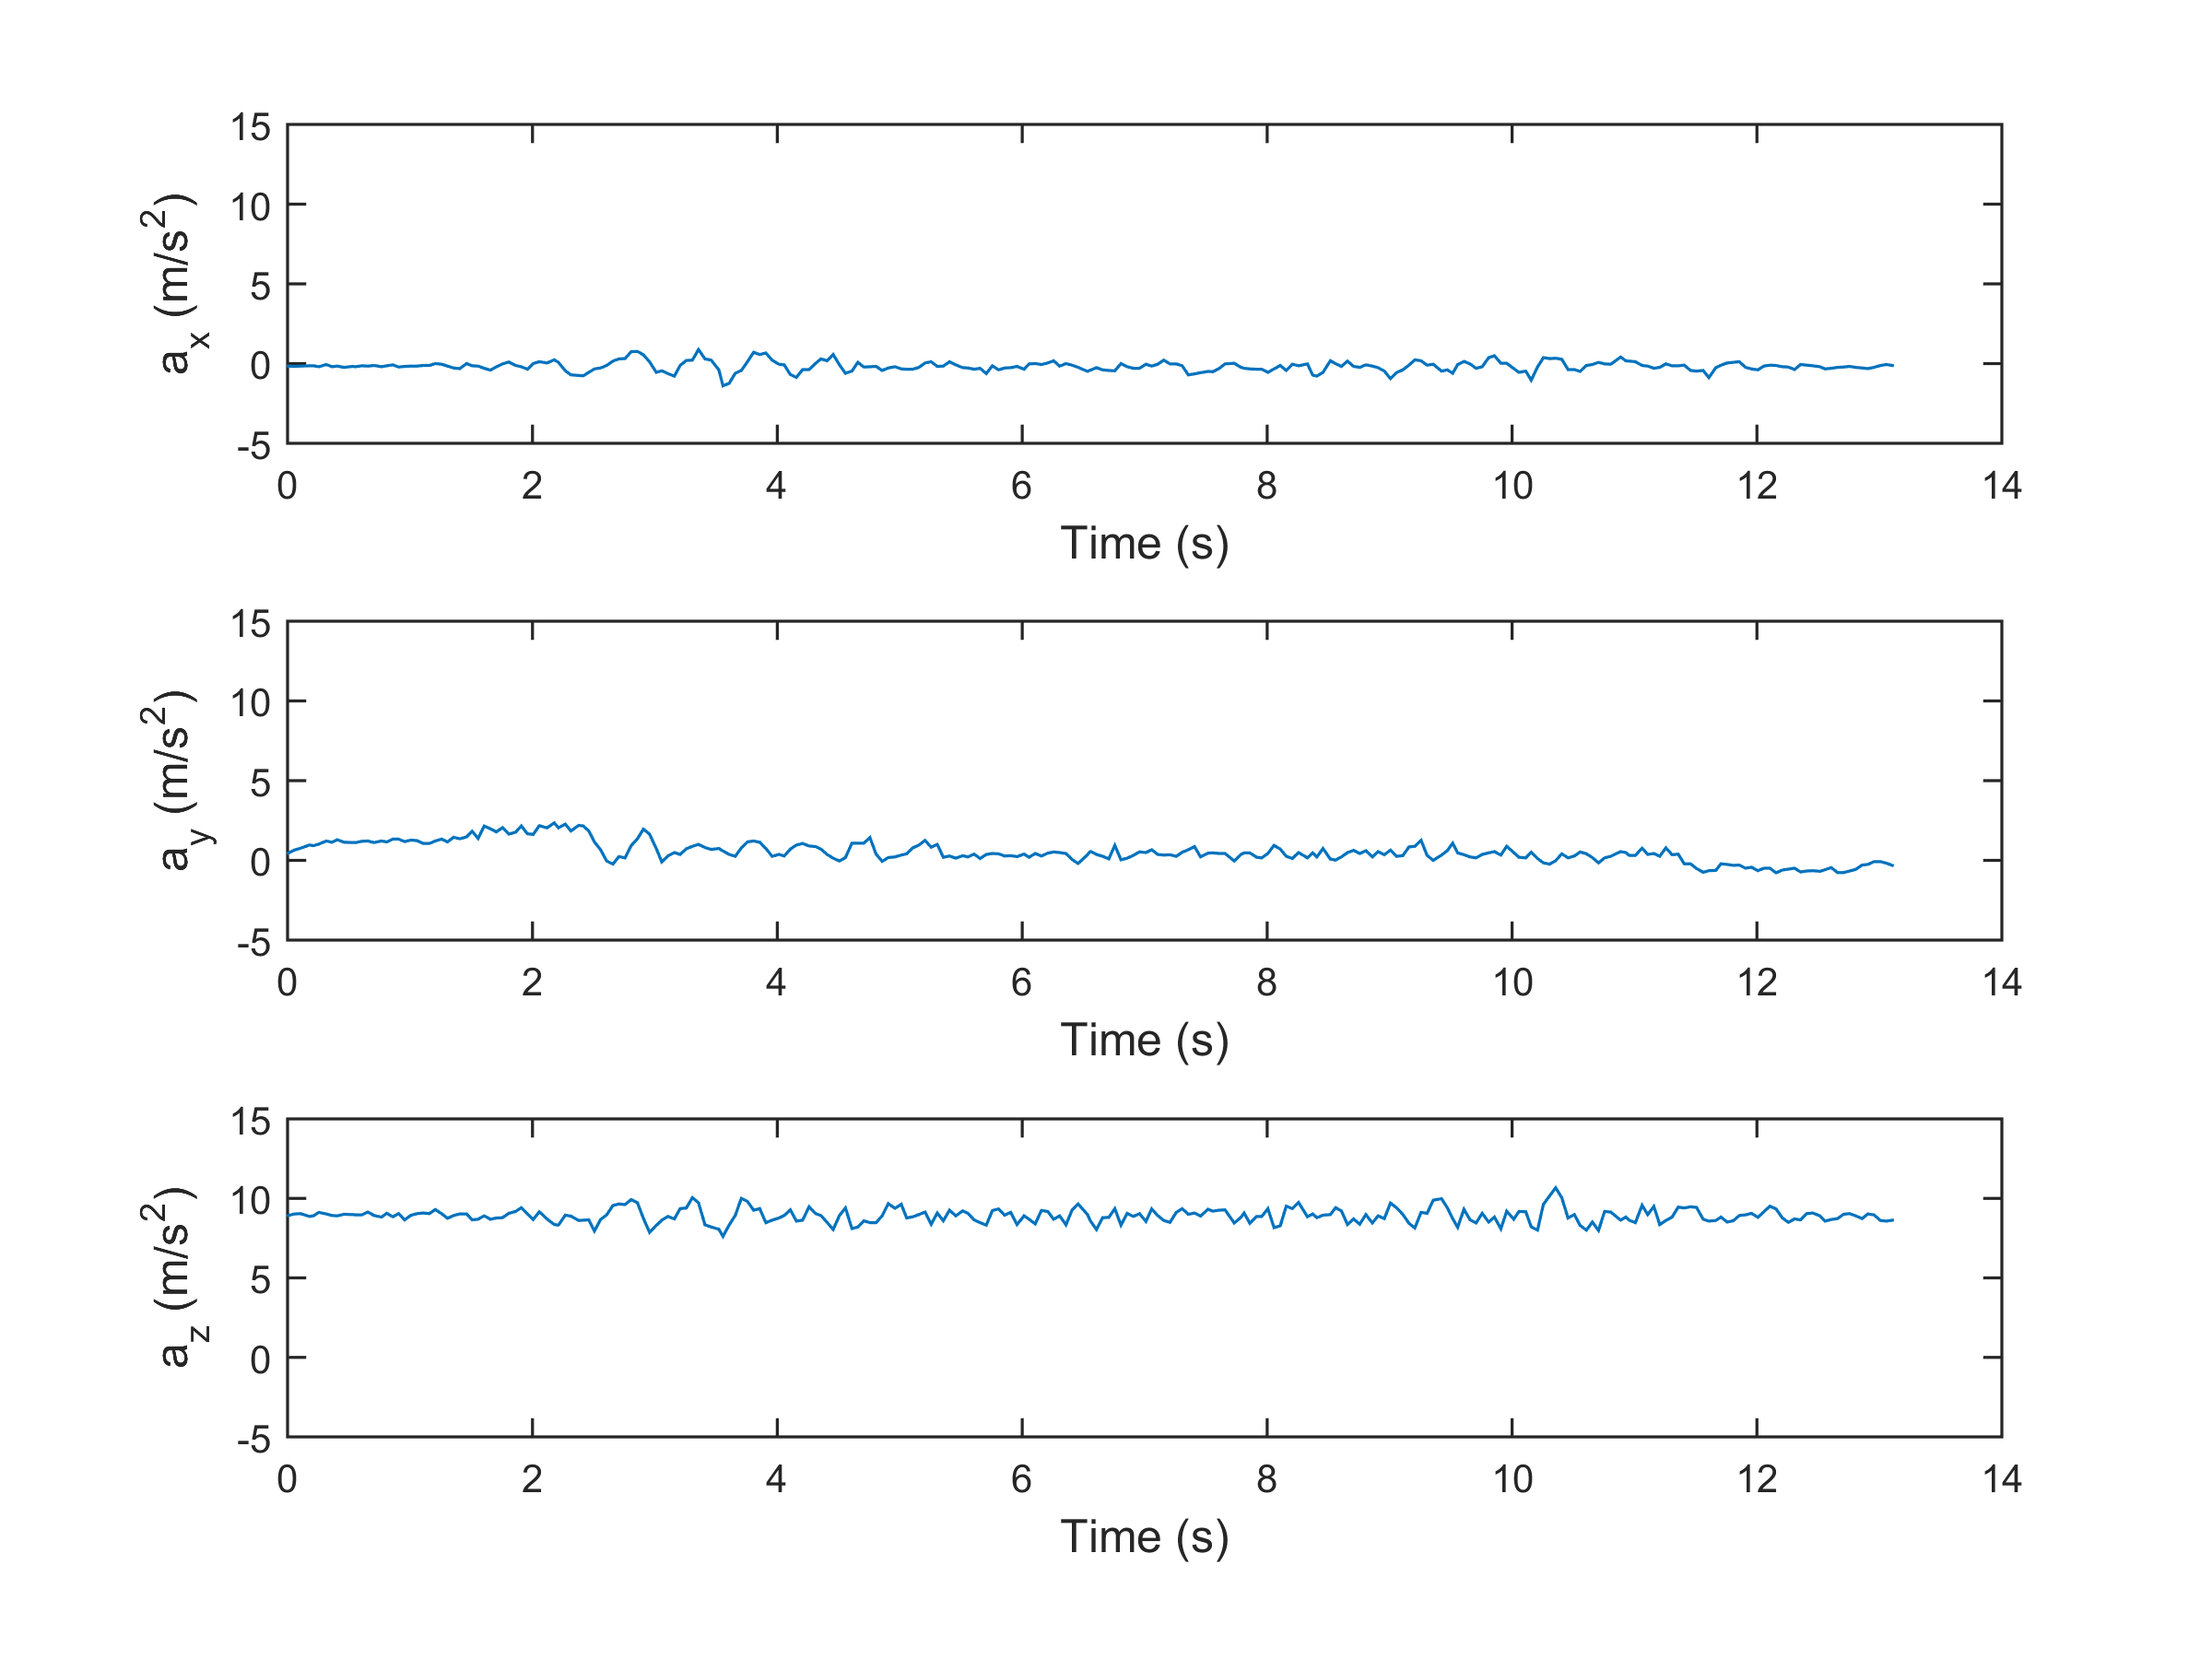
\includegraphics[scale=0.6]{figures/TypicalNormal.png}
	\caption{Typical acceleration data when the test vehicle crosses a road without road anomalies.}
	\label{fig:TypicalNormal}
\end{figure}

Figure \ref{fig:TypicalPothole} shows acceleration data when a vehicle crosses a normal road then hits
a pothole. Region in between the sixth and eighth seconds is when the vehicle
hits the pothole. Notice that starting from the normal value of gravity
acceleration, the $z$ acceleration falls to $\text{5--7 m/s}^2$. It is when the front wheel
hits the base of the pothole. After that the $z$ acceleration starts to rise
significantly to $\text{12--13 m/s}^2$. It is when the front wheel exits the pothole. The
next drop is caused by the rear wheel hitting the pothole base. Identical to the
previous one, this one is also followed by another rise when the rear wheel
exits the pothole

\begin{figure}[!b]
	\centering
	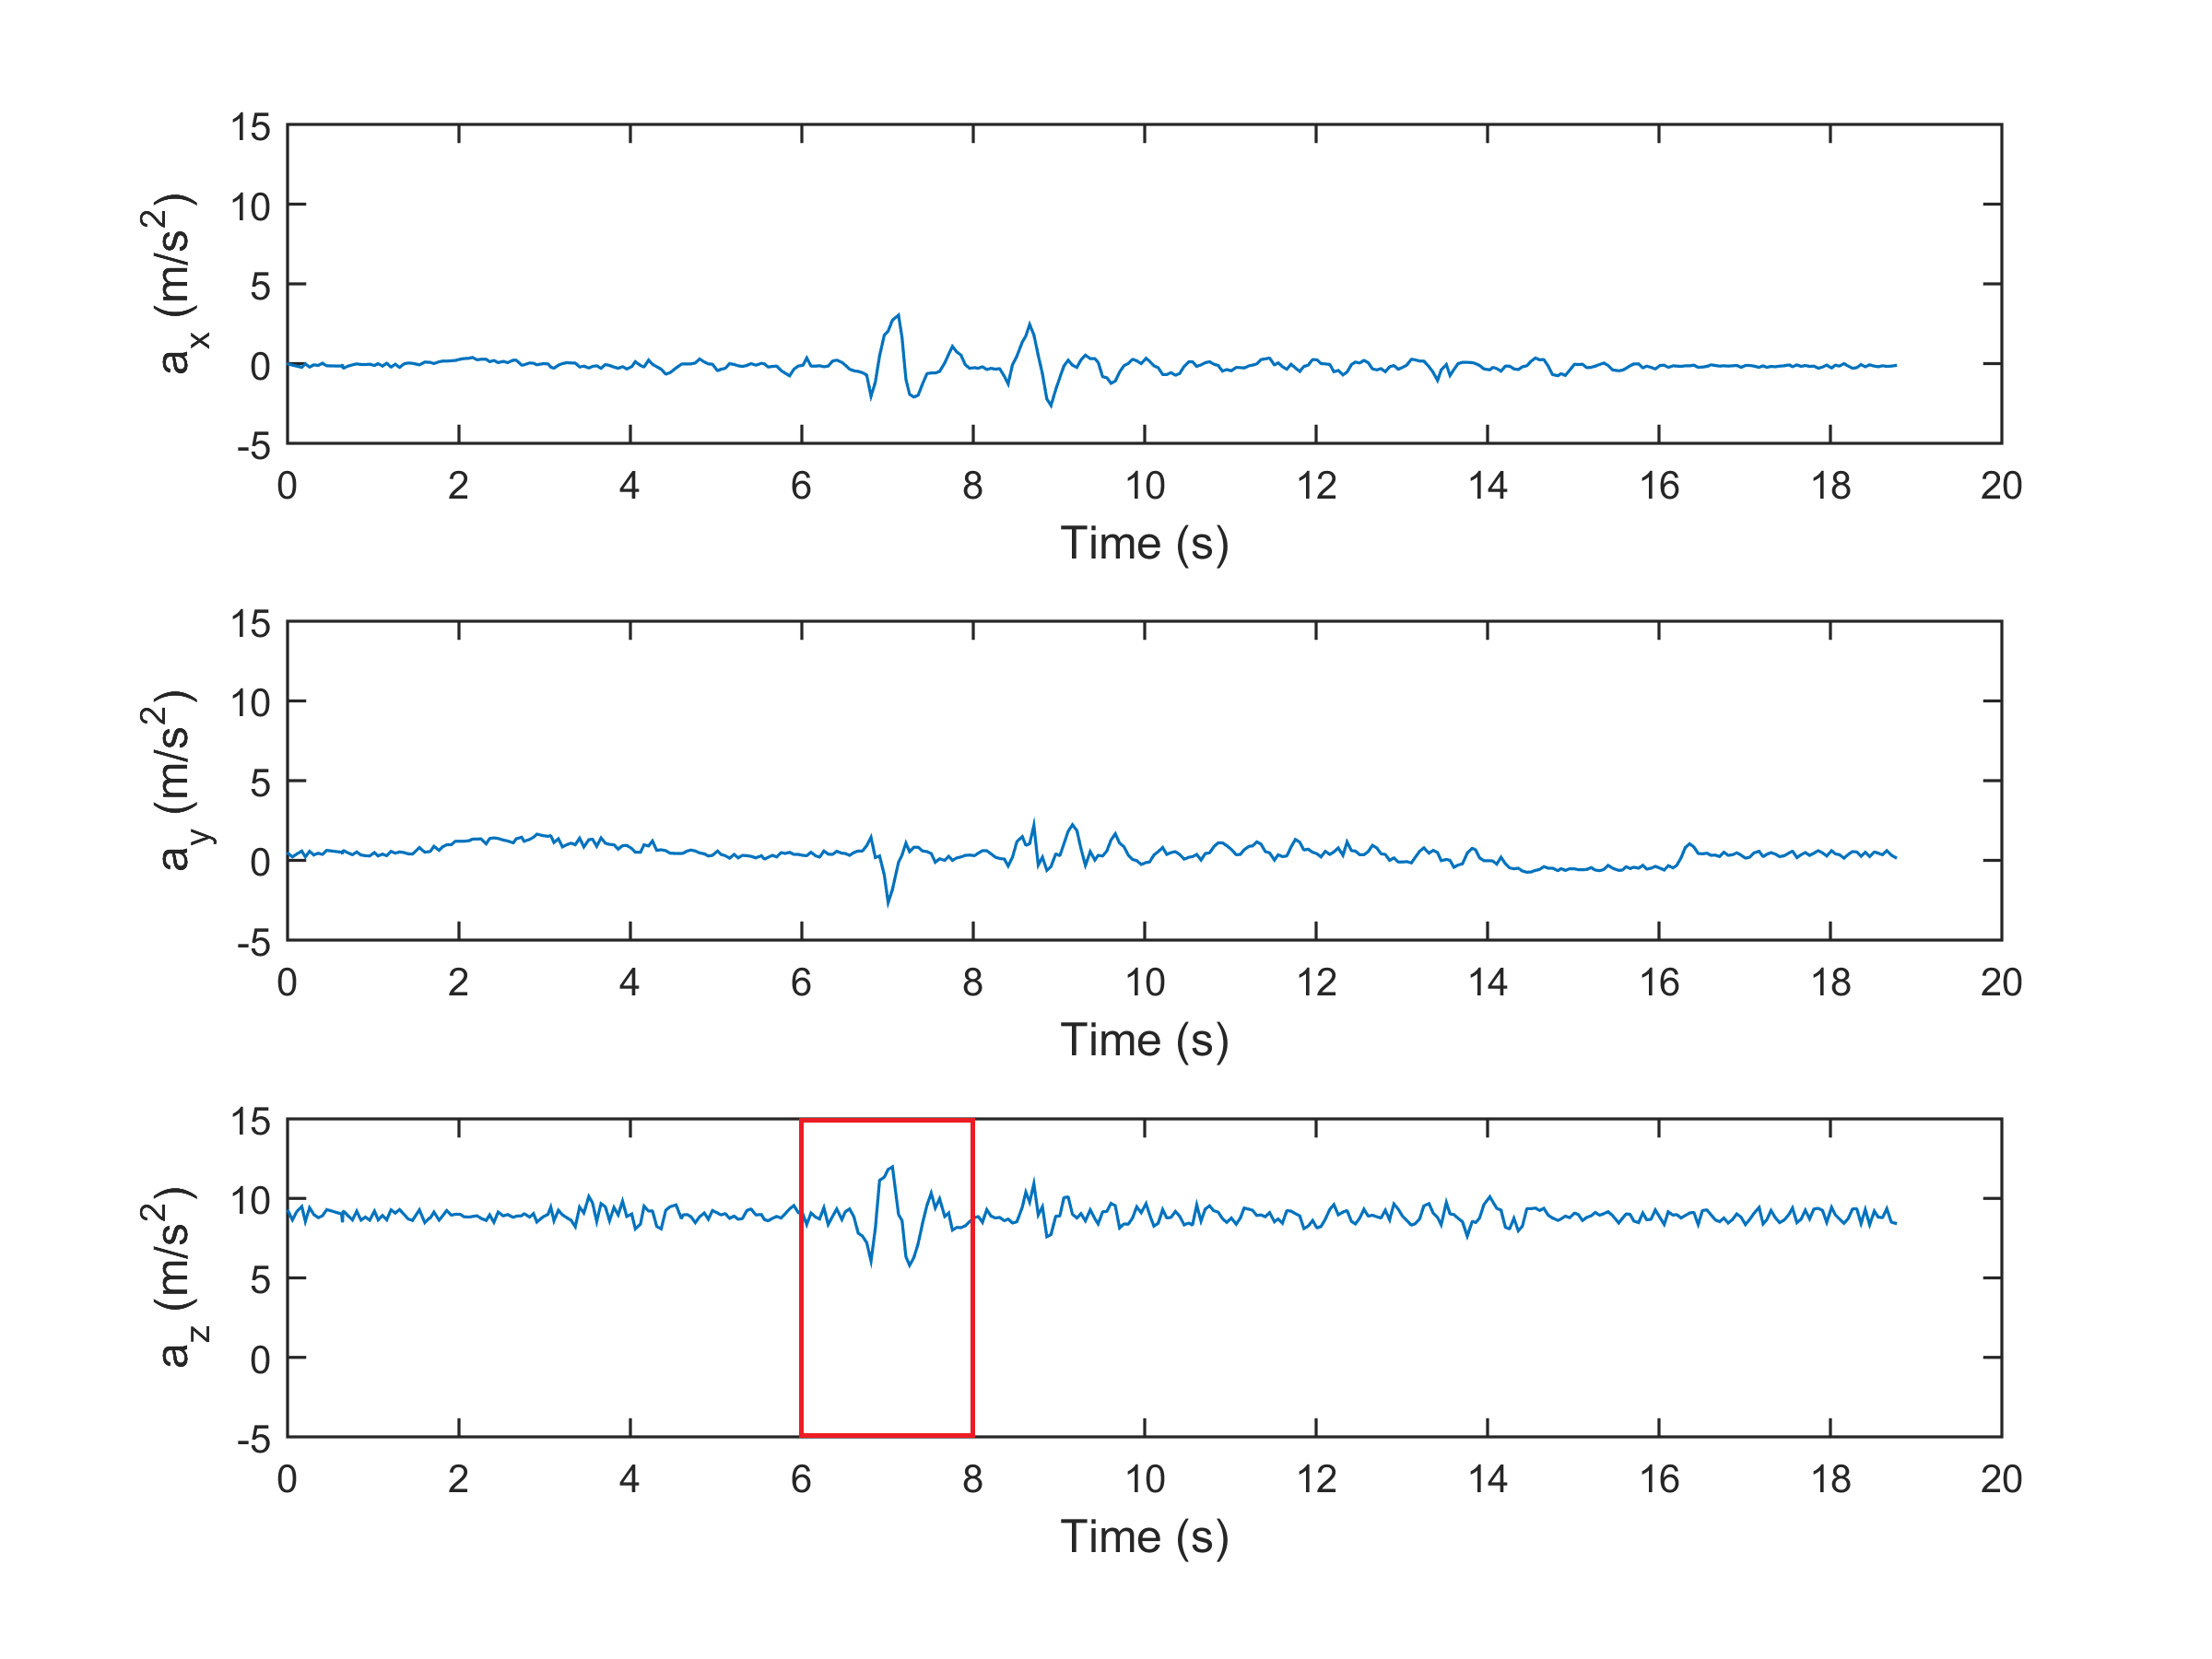
\includegraphics[scale=0.6]{figures/TypicalPothole.png}
	\caption{Typical acceleration data when the test vehicle crosses a pothole.}
	\label{fig:TypicalPothole}
\end{figure}

Figure \ref{fig:TypicalSpeedbump} shows acceleration data when a vehicle crosses a normal road then hit a
speed bump. Region in between the eleventh and thirteenth second is the time
when the vehicle hits the speed bump. When the front wheel hits the speed bump,
it gives significant increase to $z$ acceleration from gravity acceleration value
to about $\text{13-�14 m/s}^2$. After that $z$ acceleration starts to fall off because the
front wheel has passed through the speed bump.

\begin{figure}[!ht]
	\centering
	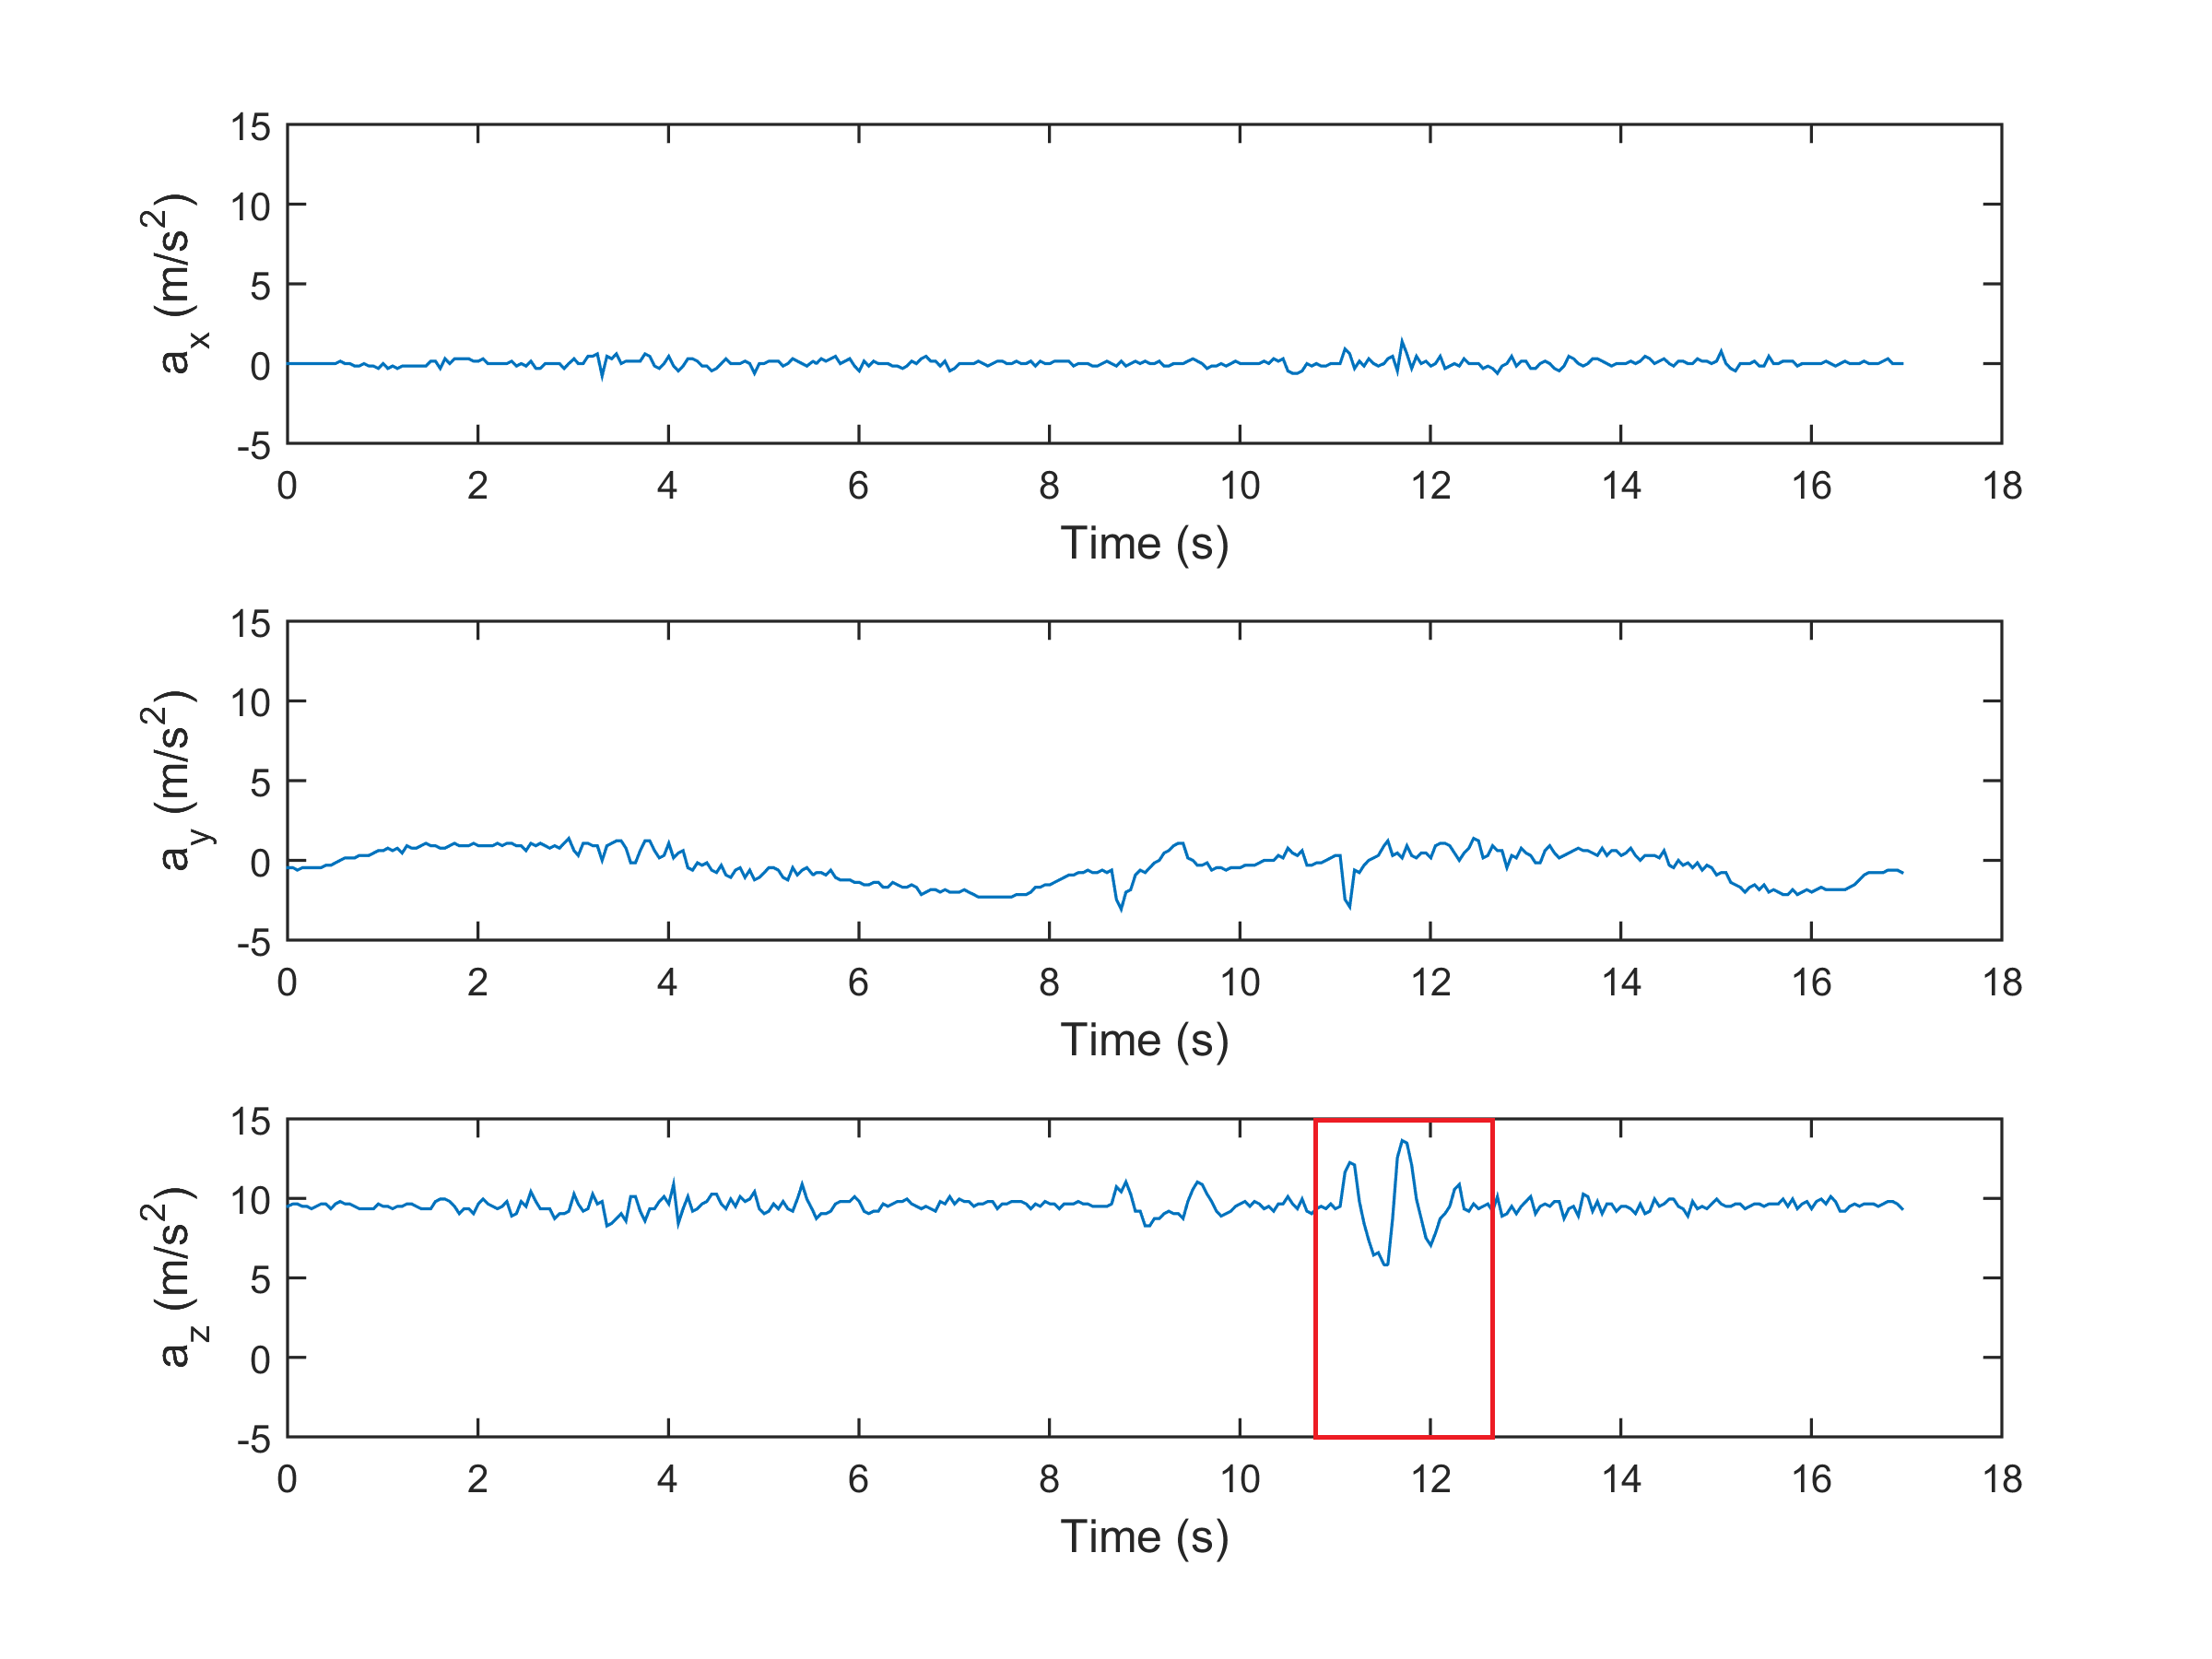
\includegraphics[scale=0.6]{figures/TypicalSpeedbump.png}
	\caption{Typical acceleration data when the test vehicle crosses a speed bump.}
	\label{fig:TypicalSpeedbump}
\end{figure}

Figure \ref{fig:TypicalExpansionJoint} shows acceleration data when a vehicle crosses a normal road then
passing an expansion joint. Region in between the fifth and sixth second is the
data recorded when the vehicle crosses the expansion joint. When the wheel hits
the expansion joint, it drops the $z$ acceleration to about $\text{7�-8 m/s}^2$. Then the $z$
acceleration rises significantly to about $\text{15 m/s}^2$.

\begin{figure}[!ht]
	\centering
	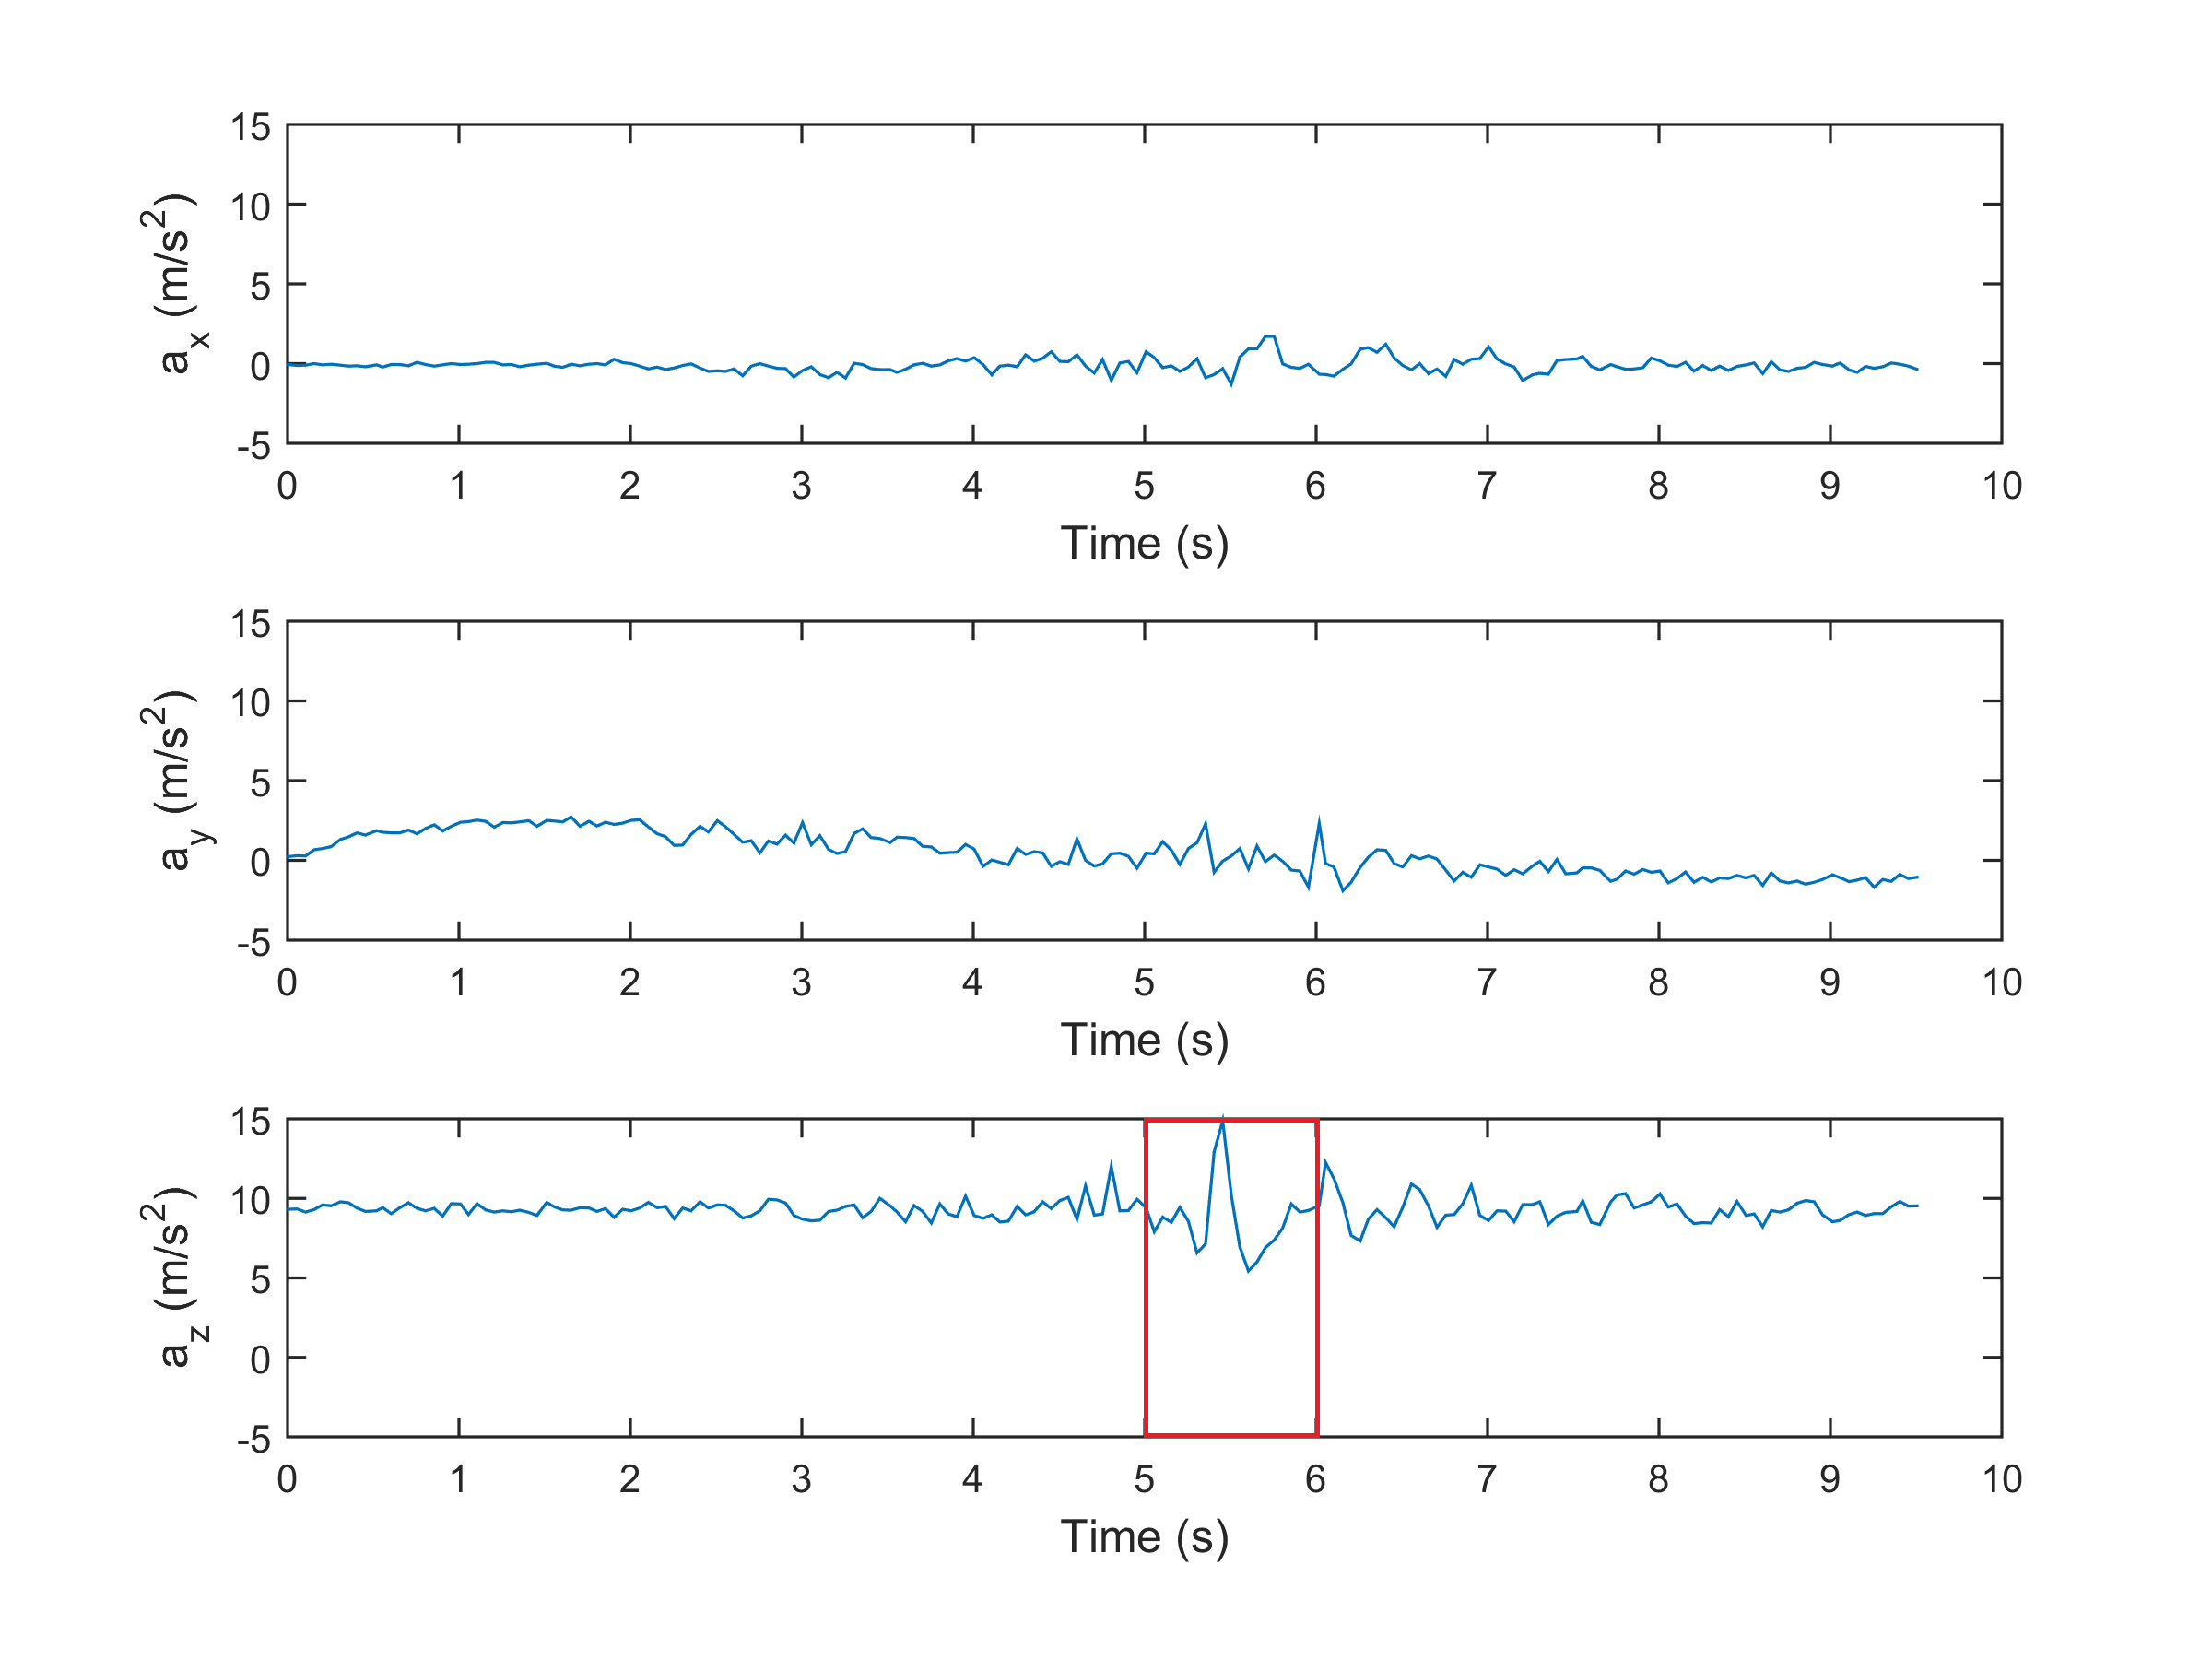
\includegraphics[scale=0.6]{figures/TypicalExpansionJoint.png}
	\caption{Typical acceleration data when the test vehicle crosses a speed bump.}
	\label{fig:TypicalExpansionJoint}
\end{figure}


\subsection{Determining the Reliable Sample Size}
This study evaluates a variation of the training data size to the accuracy of
the ANN prediction. The approach is of the following. Firstly, the training size
is fixed at 10\% of the total sample size. The remain data are equally divided
for the validation and testing stages. For these fixed sizes, the data are
resampled for a hundred times using a Monte Carlo simulation. This procedure is
repeated for the training size of 20\%, 30\%, ..., 80\% and 90\%.
\par The effects of the data sizes on the accuracy are shown in Figure \ref{fig:PercentageTrainingDataResult}. The
ANN model trained using 10\% data is only about 15\% accurate or about 85\%
misclassify the cases. The accuracy increases almost steadily with the
increasing of the training data size until the data size reaches 50\%. After the
size, the accuracy still slightly varies with the data size. The highest
accuracy is obtained for 80\% training data size.

\begin{figure}[!b]
	\centering
	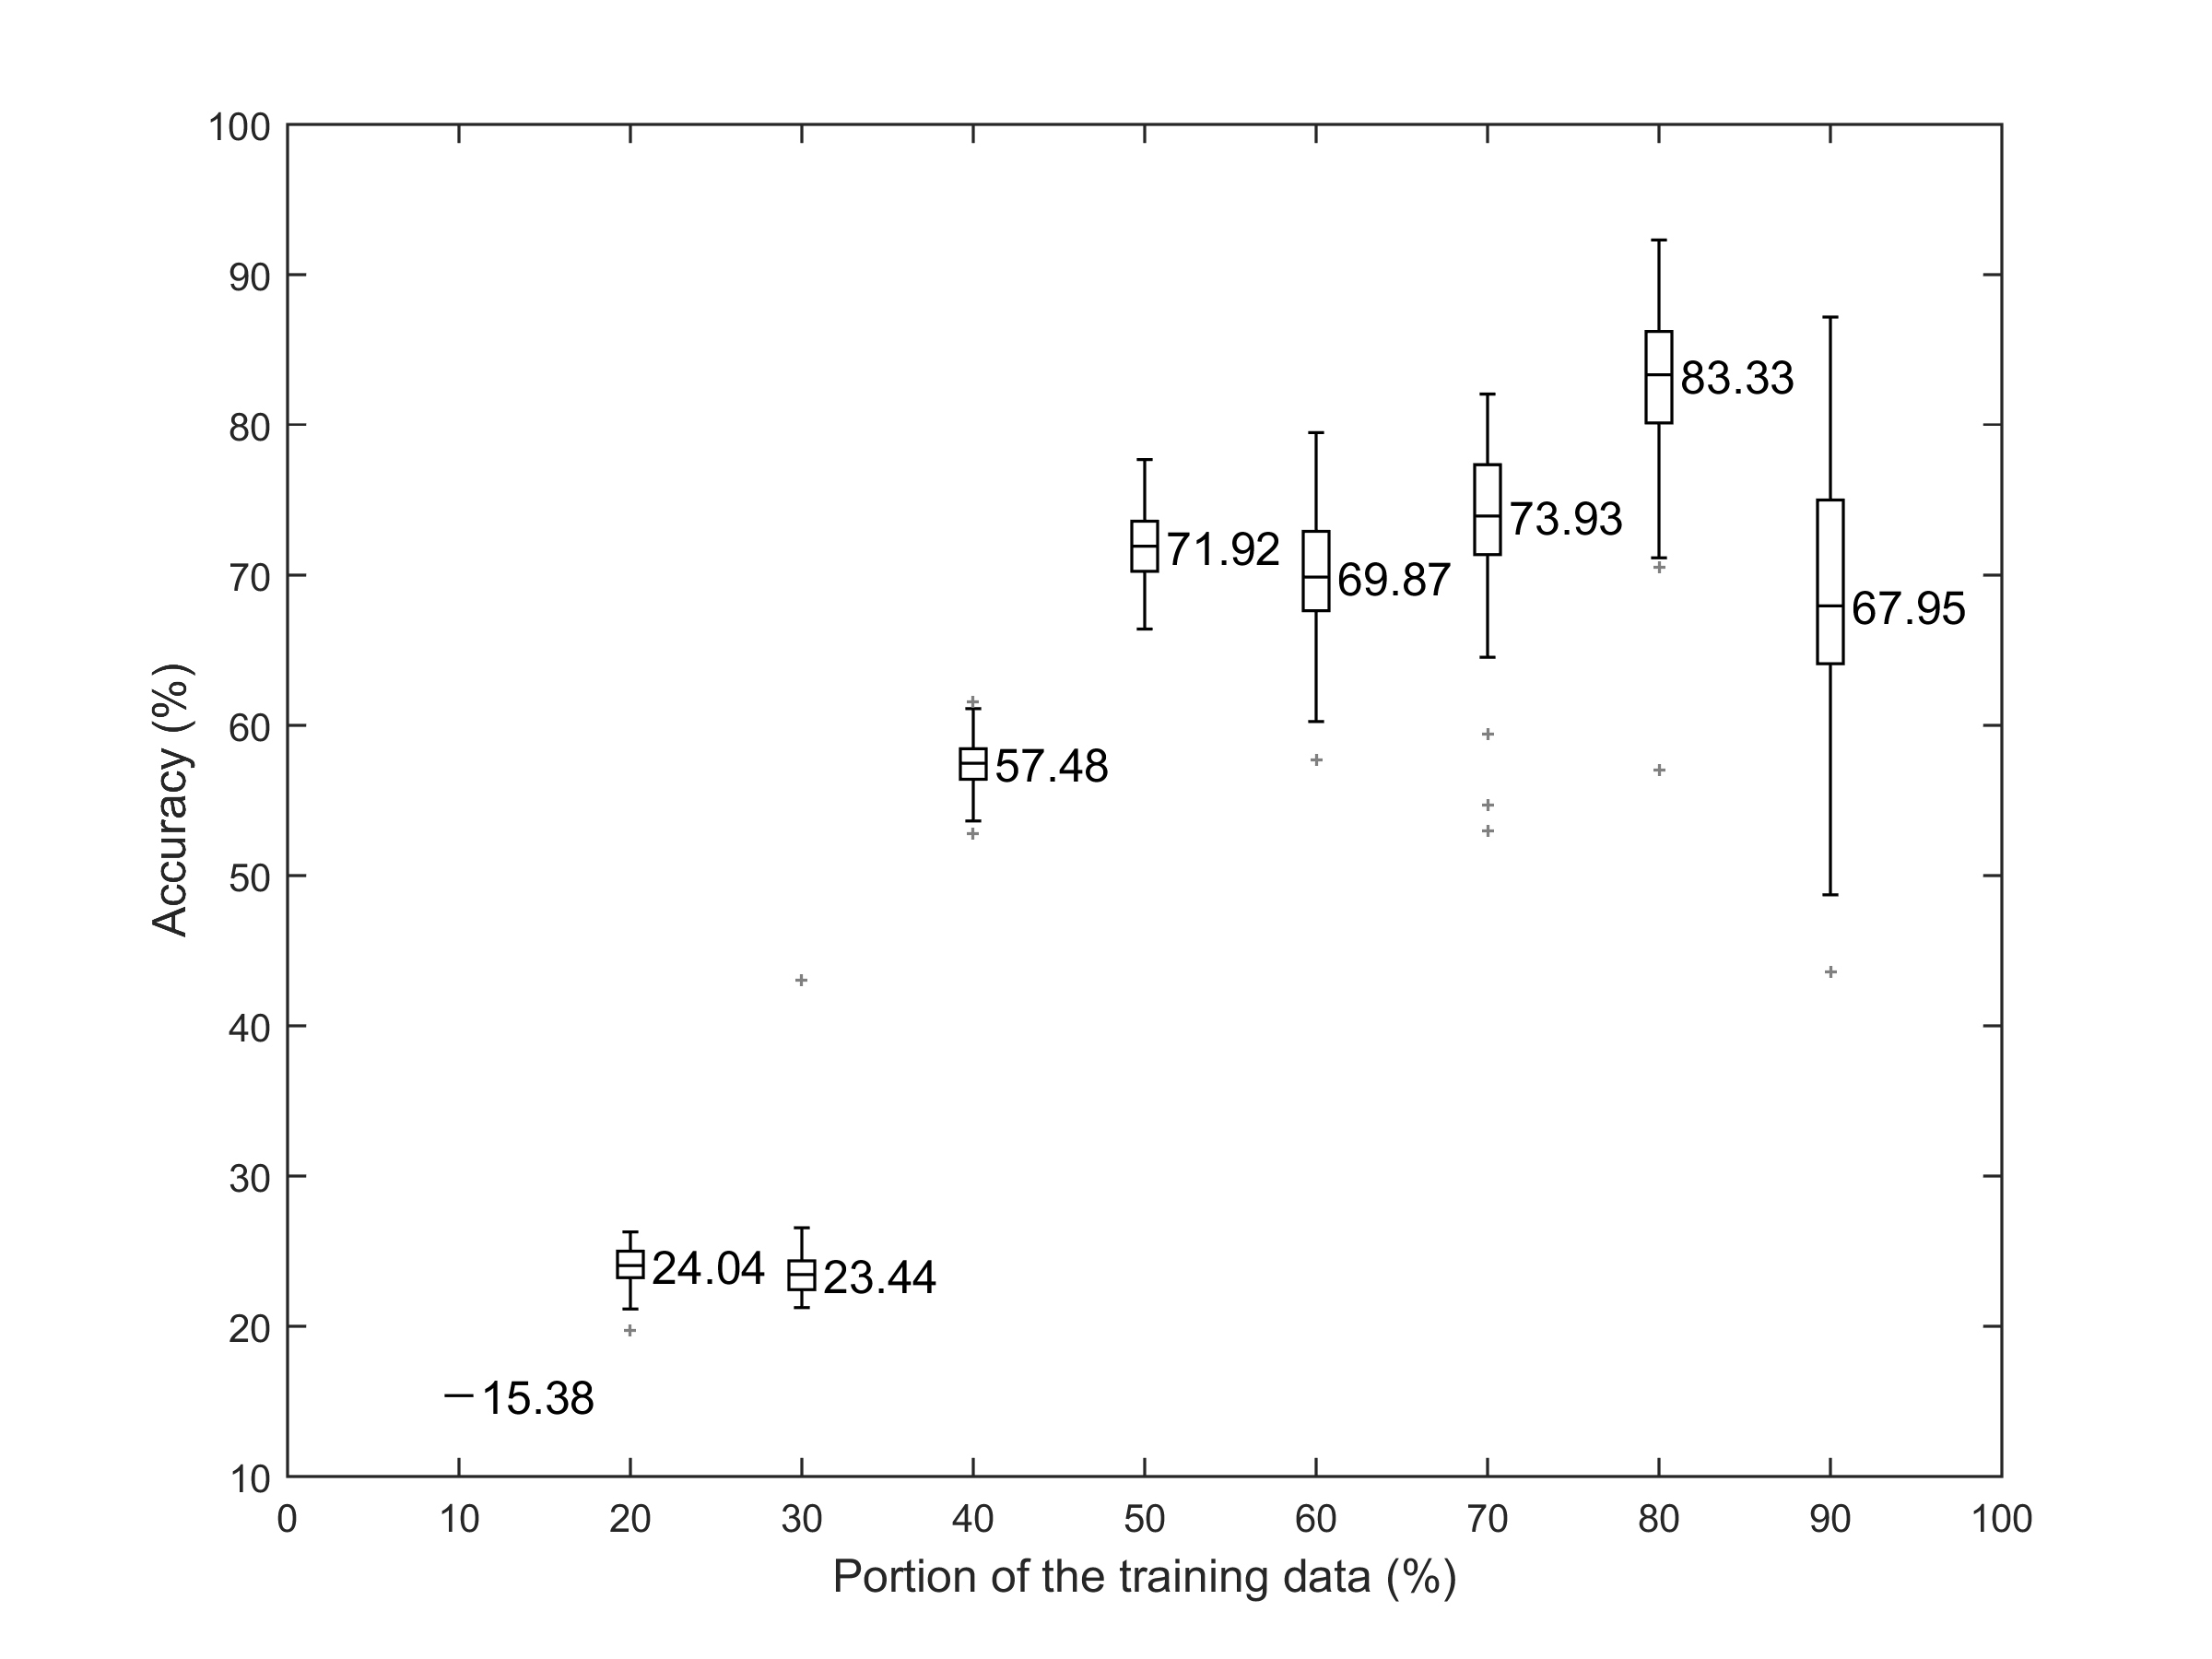
\includegraphics[width=1\linewidth]{figures/PercentageTrainingDataResult.png}
	\caption{The effects of the portion of the training data to the classification accuracy of the road anomalies.}
	\label{fig:PercentageTrainingDataResult}
\end{figure}

\subsection{Determining the Optimum Number of Neurons}
Increasing the number of neurons increases the capability of the model to fit
more complex relationship. However, this complexity may happen due to over
fitting. A good ANN network model should be general and not overfit to a
specific case. A minimum number of neurons is usually required to provide a
generic model.
To find this generic model, the neural model accuracy is computed for a various
number of neurons. The results are depicted in Figure \ref{fig:NumberofHiddenLayerResult}. For the two-neuron
case, the accuracy varies widely from around 57\% up to around 91\%. However, for
the cases where the number of neurons is three and nine, the accuracy variation
is relatively constant from one case to the others. The figure suggests that the
most optimum number of neurons is three.

\begin{figure}[!b]
	\centering
	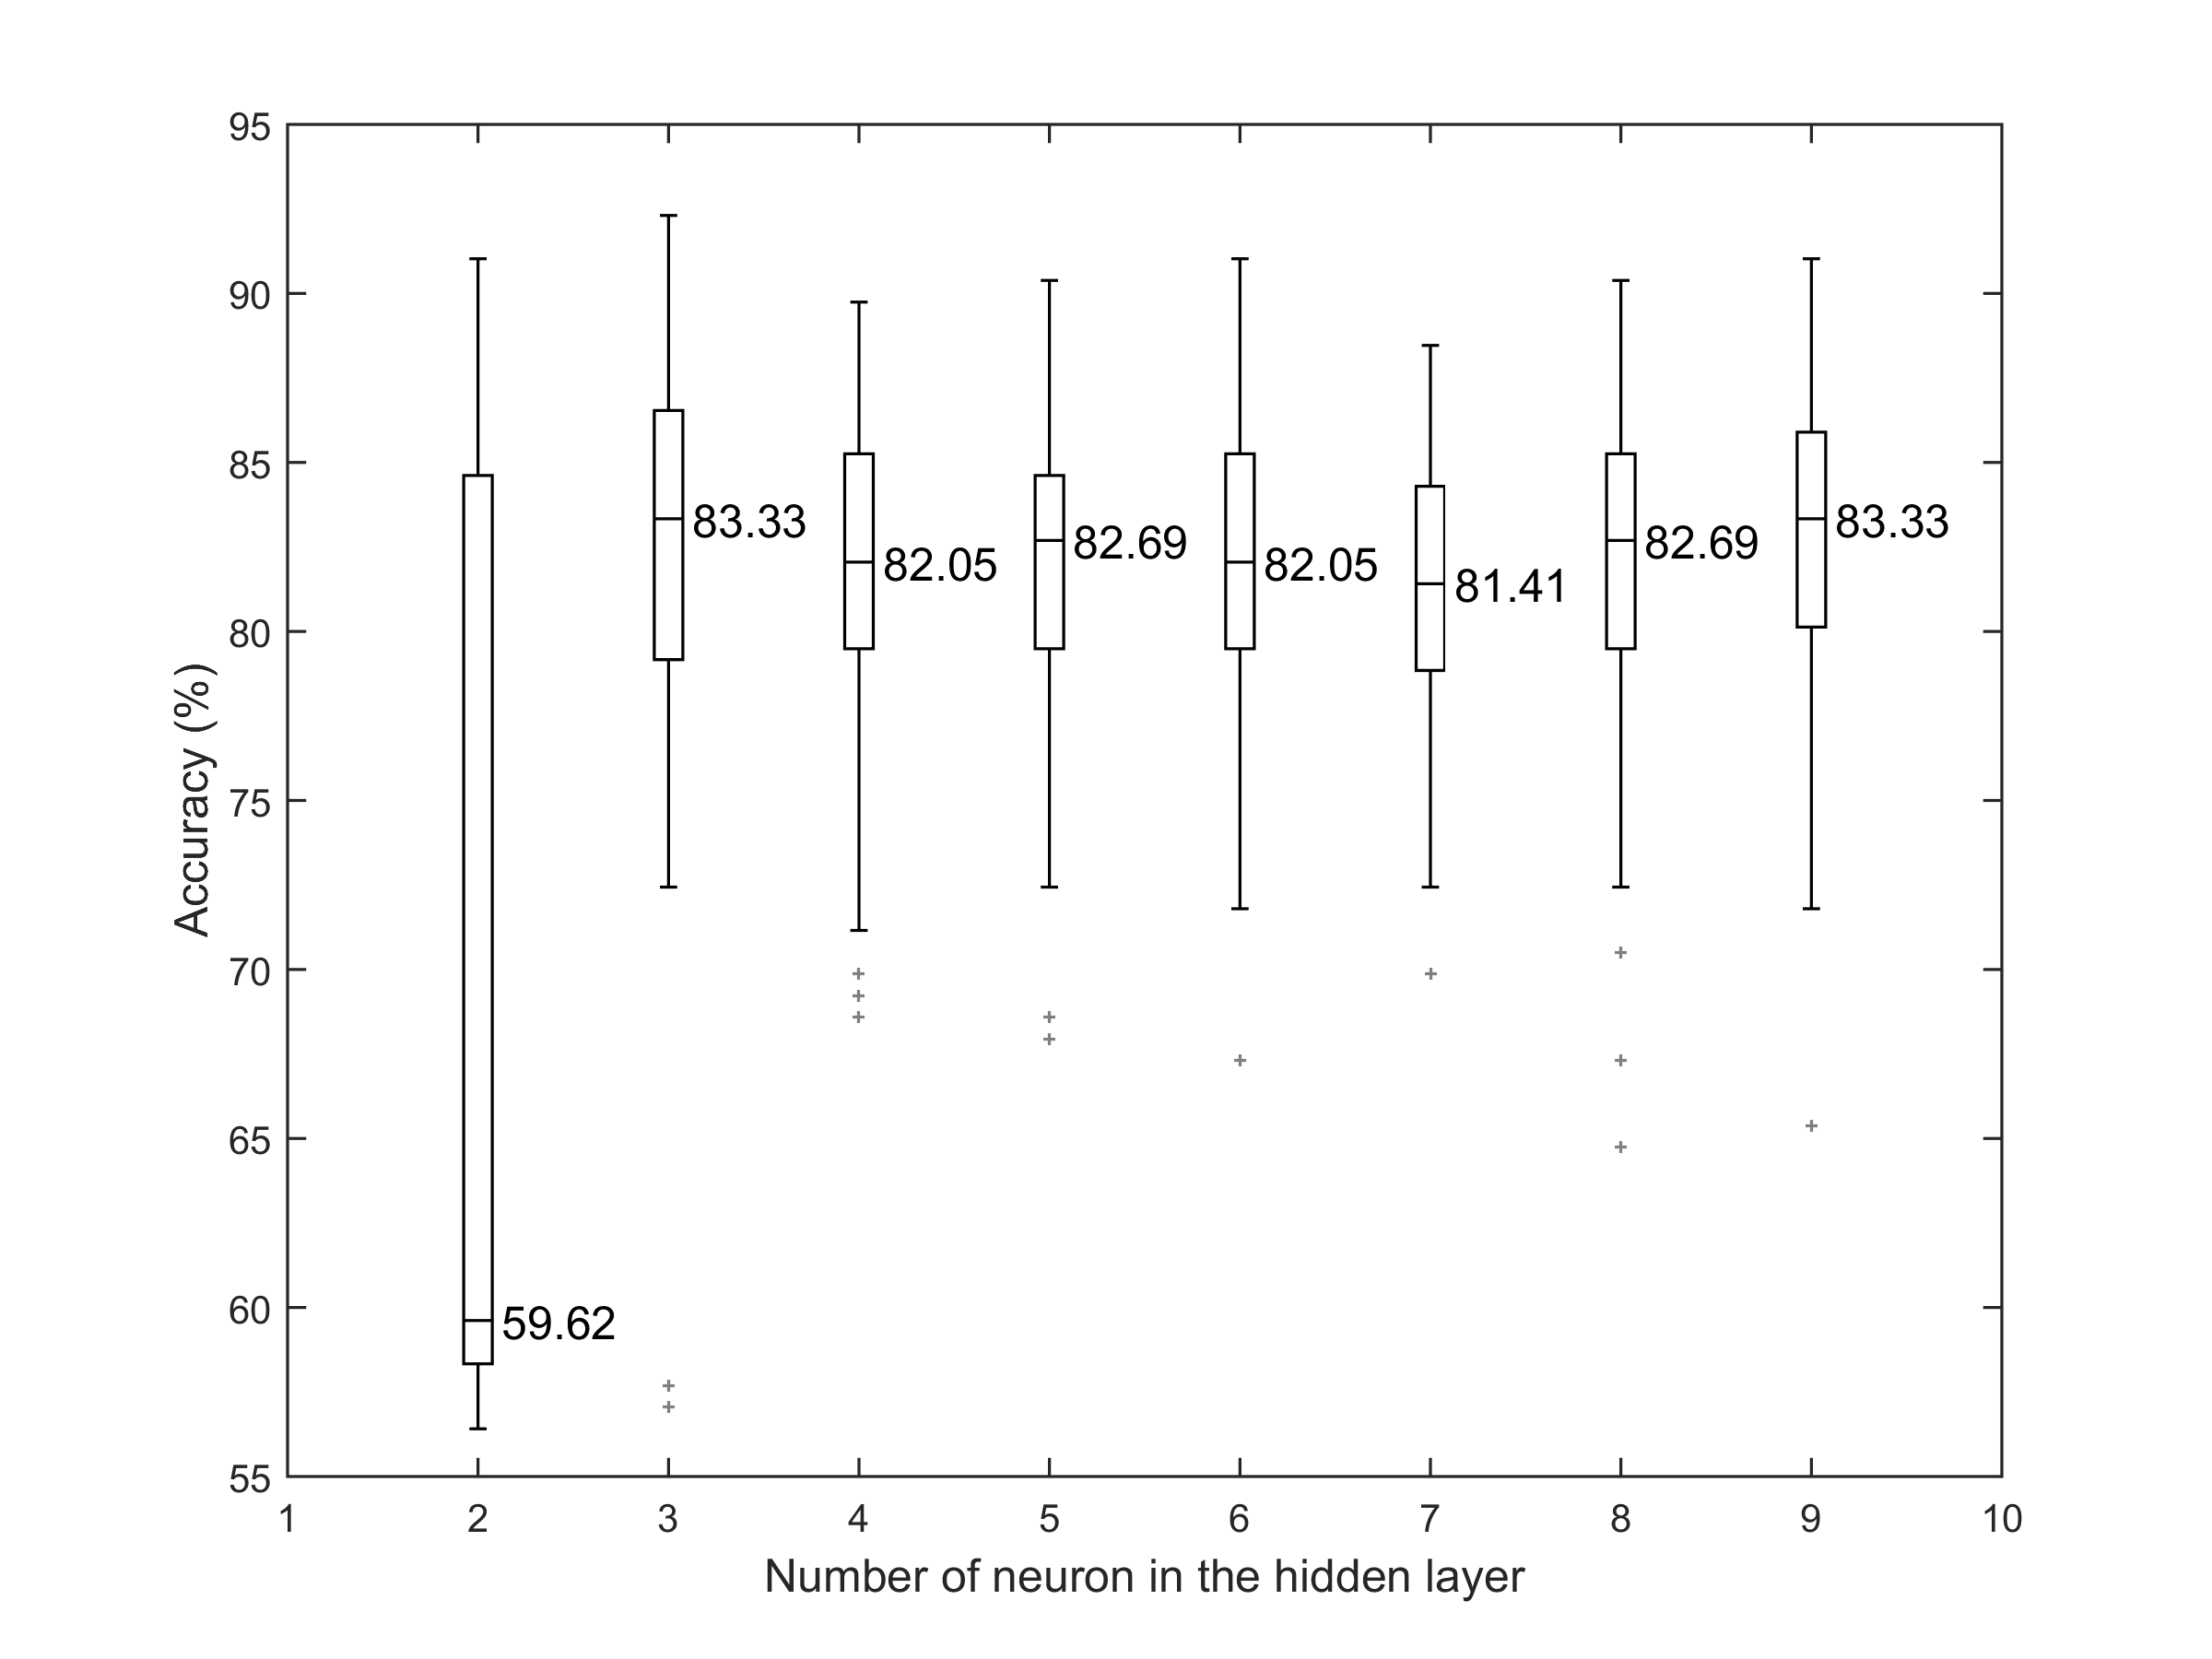
\includegraphics[width=1\linewidth]{figures/NumberofHiddenLayerResult.png}
	\caption{The effect of the number of neurons in the hidden layer to the classification accuracy of the road anomalies.}
	\label{fig:NumberofHiddenLayerResult}
\end{figure}

\subsection{Determining the Significance Features}
Feature selection is the process of selecting a subset of relevant features for
use in the classifier model construction. Sometimes the data collected may
redundant or irrelevant. Features selection may help eliminate this possibility
by preventing loss of information. Theoretically, smaller number of features can
decrease the classifier workload, hence decreasing the modelling and training
time of the classifier. This also increases the classifier performance by
maintaining its accuracy. To perform feature selection, the condition of the
data in each class must firstly be observed. The distribution of features of the
classification is shown in  Figure \ref{fig:BoxPlotFeaturesDistribution}.

\begin{sidewaysfigure}
	\centering
	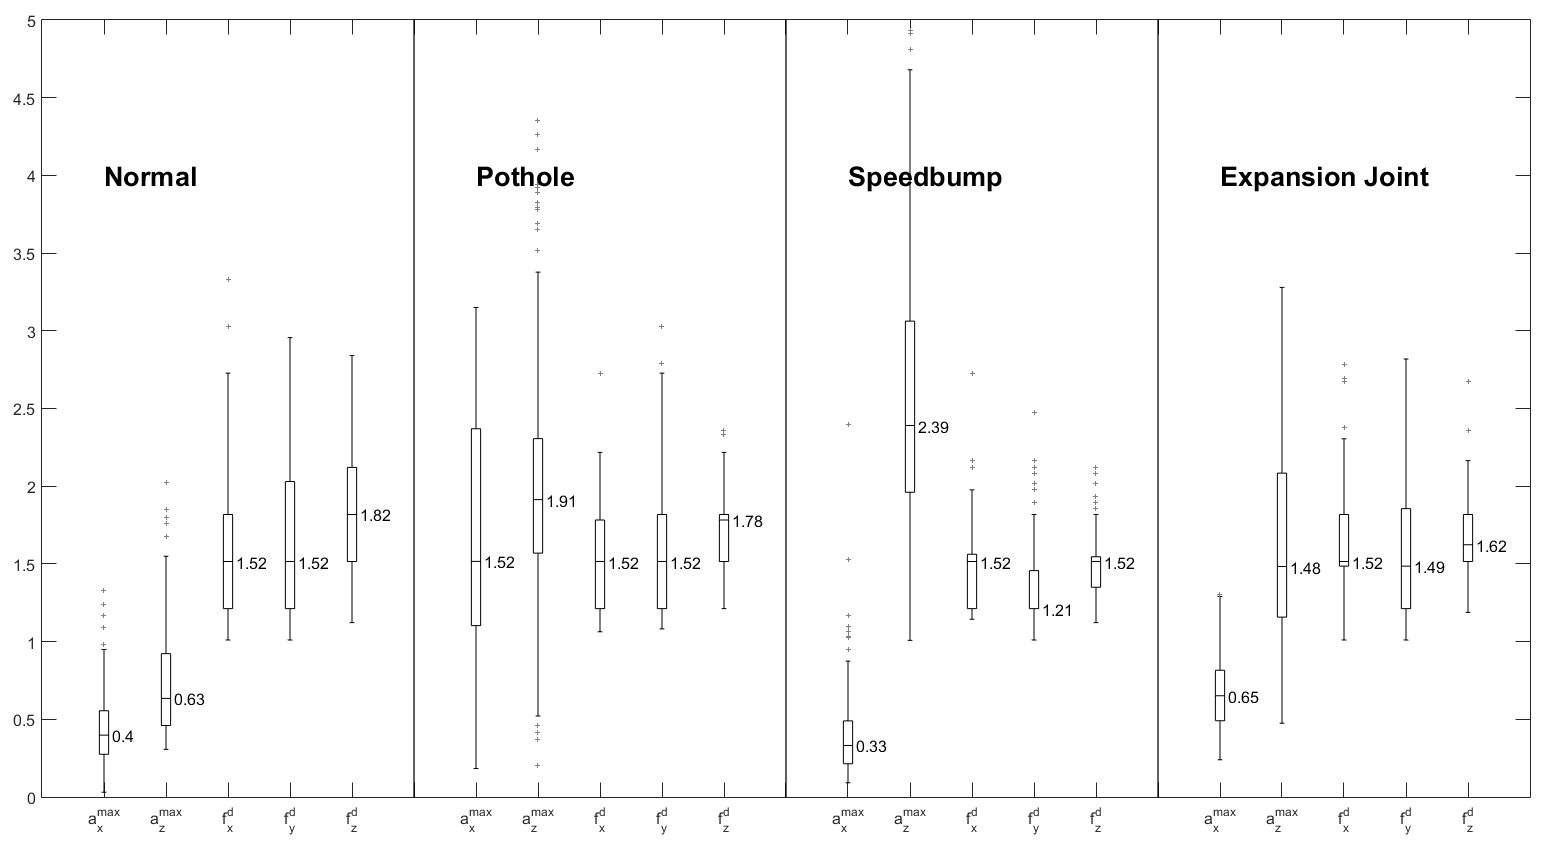
\includegraphics[scale=0.7]{figures/BoxPlotFeaturesDistribution.png}
	\caption{The features distribution for each class in this classification.}
	\label{fig:BoxPlotFeaturesDistribution}
\end{sidewaysfigure}

\par The dominant frequency of $x$ in normal class is 1.52, which is identical
in other classes too. Meanwhile, the dominant frequency of $y$ in normal and
pothole case both has score 1.52, while speedbump and expansion joint have 1.21
and 1.49. Only the dominant frequency of $z$ that has varied score for each
class.
\par Using these facts, further classification is performed by reducing the
number of features involved in the classifier. Table
\ref{tab:CombinationFeature} shows which features presence in each classifier.
Each classifier used 80\% training data and three neurons in the hidden layer.
This classifier is resampled for a hundred times using a Monte Carlo simulation.

\begin{table}[!b]
	\centering
	\caption{The Combination of Features Studied in The Research.}
	\label{tab:CombinationFeature}
	\resizebox{0.6\textwidth}{!}{	
	\begin{tabular}{ccccccc}
		\toprule
		\multirow{2}[3]{*}{Case} & \multicolumn{6}{c}{Features} \\
		\cmidrule(lr){2-7}
 		  & \textbf{$a^{\text{max}}_{x}$} & \textbf{$a^{\text{max}}_{y}$} & \textbf{$a^{\text{max}}_{z}$} & \textbf{$f^{\text{dom}}_{x}$} & \textbf{$f^{\text{dom}}_{y}$} & \textbf{$f^{\text{dom}}_{z}$}\\
		\midrule
		A & \checkmark & \checkmark & \checkmark & \checkmark & \checkmark & \checkmark\\
		B &			   & \checkmark & \checkmark & \checkmark & \checkmark & \checkmark\\
		C & \checkmark & 			& \checkmark & \checkmark & \checkmark & \checkmark\\
		D & \checkmark & \checkmark & 			 & \checkmark & \checkmark & \checkmark\\
		E & \checkmark & \checkmark & \checkmark & 			  & \checkmark & \checkmark\\
		F & \checkmark & \checkmark & \checkmark & \checkmark & 		   & \checkmark\\
		G & \checkmark & \checkmark & \checkmark & \checkmark & \checkmark & 		   \\
		H & \checkmark & \checkmark & \checkmark & 			  & 		   & 		   \\
		\bottomrule
	\end{tabular}}
\end{table}

\par After testing the classifier, the results are depicted in Figure \ref{fig:ComparisonofANNVariedFeatures}. Classifier
A that used all the features has accuracy of 85.2\%. Classifier B has 46.1\%
accuracy, which is the worst amongst another classifier. Classifier B did not
include $a^{\text{max}}_{x}$ as its features. From this result can be predicted that $a^{\text{max}}_{x}$
is a significance features.

\begin{figure}[!ht]
	\centering
	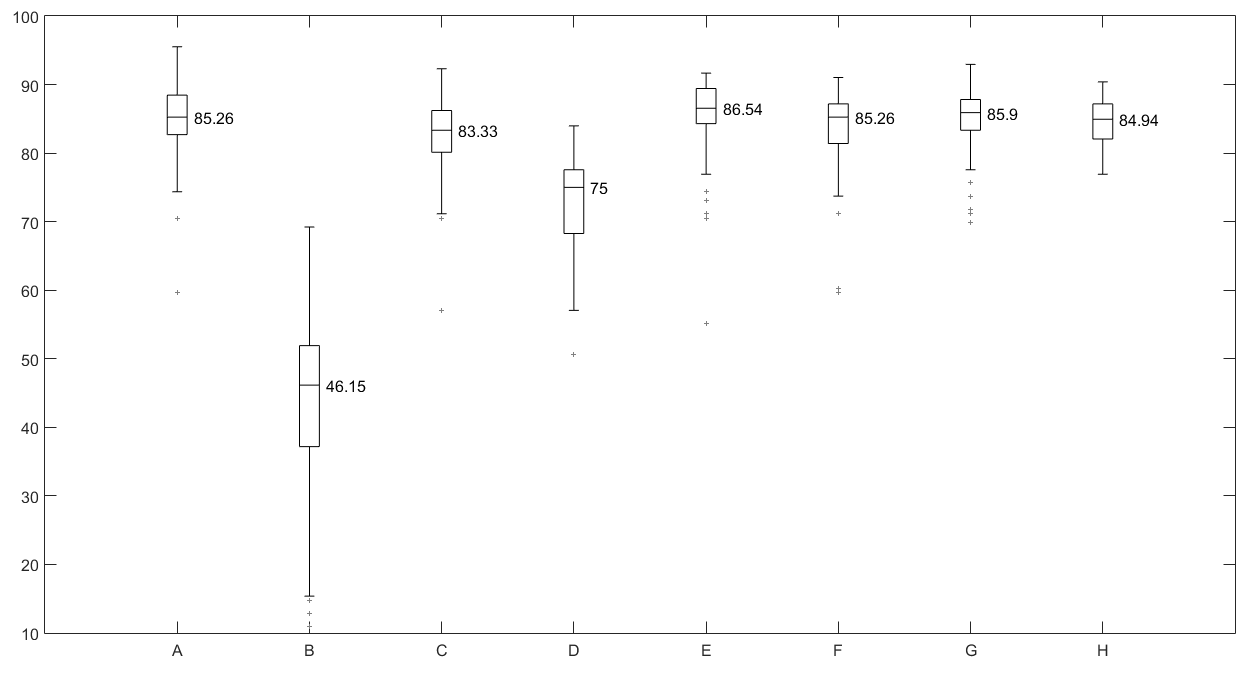
\includegraphics[scale=0.4]{figures/ComparisonofANNVariedFeatures.png}
	\caption{The classification accuracies in percent for various combinations of features.}
	\label{fig:ComparisonofANNVariedFeatures}
\end{figure}

\par Classifier C accuracy is 83.3\%. Its accuracy is slightly lower than classifier
A. This classifier did not have $a^{\text{max}}_{y}$ as its feature. Meanwhile Classifier D
has second lowest accuracy at 75\% and missing $a^{\text{max}}_{z}$. Removing maximum
acceleration reduce the performance of the classifier.

\par Classifier E, F, and G remove dominant frequency of the acceleration data from
its features. Interestingly, the three of them have similar result with
classifier A which is include all of them. The accuracy tends to stay at 85--86\%.
This may become indicator that dominant frequency is not a significance
features.

\par Lastly, classifier H that used $a^{\text{max}}_{x}$, $a^{\text{max}}_{y}$, and $a^{\text{max}}_{z}$ as its
features perform at 84.9\% accuracy. This score is 0.3\% smaller than classifier A
which includes all features. This is a prove that frequency data may not be
required as the features for the classification model.



% %CHAPTER 4
% %=============================================================================================
\section{Conclusion}
The focus of this research is finding the best features to classify road
anomaly, which categorized into four classes: normal, pothole, speedbump, and
expansion joint within artificial neural network framework and measures its
performance. The results have been presented and discussed in the previous
chapter. The following are the conclusions:
\begin{enumerate}
  \itemsep 0em
  \item The most optimum size of training data  for the ANN model is 80\%.
  \item The most optimum number of neurons of the ANN model is three.
  \item The most optimum features are maximum x acceleration, maximum z acceleration and maximum z acceleration with accuracy of 84.9\%.
  \item Dominant frequency of each acceleration data was predicted to be a significance features. However the result proves that these features do not rise the accuracy significantly. Removing each give 88.5\%, 85.2\%, and 85.9\% accuracy respectively, which is slightly greater than using acceleration data only which is 84.9\%.
\end{enumerate}
%%=============================================================================================


%% The Appendices part is started with the command \appendix;
%% appendix sections are then done as normal sections
%% \appendix

%% \section{}
%% \label{}

%% References
%%
%% Following citation commands can be used in the body text:
%% Usage of \cite is as follows:
%%   \cite{key}         ==>>  [#]
%%   \cite[chap. 2]{key} ==>> [#, chap. 2]
%%

%% References with BibTeX database:

\bibliographystyle{IEEEtran}
\bibliography{references}

%% Authors are advised to use a BibTeX database file for their reference list.
%% The provided style IEEEtran.bst formats references is generally used.


\end{document}

%%
%% End of file `telkomnika.tex'. 